%%%--------------------------------%%%
%%% Domain
%%%--------------------------------%%%
\newpage
\section{Software Specification}
\label{sec:domainB}

\subsection{Purpose and Scope}
\label{sec:domainBa}
What is the software for and what is not part of the project (I'm integrating the vision part here because I don't think we need to state why we describe requirements)

\subsection{Functionalities}
\label{sec:domainBb}
Basically just the \ac{UC}

\subsubsection{Overall Use Case Diagram}
\label{sec:domainBba}


\newpage
% UC1 ====================================================
\subsubsection{Use Case Specification: \ac{UC}1 User CRUD}
\label{sec:domainBbb}

\paragraph*{Description}\mbox{}\\
Describe the functionality

\paragraph*{Screenshots}\mbox{}\\
Insert screenshots and shortly explain what can be seen
\begin{figure}[h] 
	\centering
	
\includegraphics[width=0.1\textwidth]{Content/Domain/placeholder.png}
	\caption{Use Case X: Detail}
	\label{fig:useCaseXDetailY}
\end{figure}

\paragraph*{Basic Flow} \mbox{}\\

Describe the most common path through this use case

\subparagraph{Activity Diagram}\mbox{}\\
\begin{figure}[h]
	\centering
	
\includegraphics[width=0.1\textwidth]{Content/Domain/placeholder.png}
	\caption{Activity Diagram Use Case X}
	\label{fig:activityDiagramX}
\end{figure}

\paragraph*{Alternative Flows}\mbox{}\\
What can go wrong :D

\paragraph*{Special Requirements and Preconditions}\mbox{}\\
Where does the user come from, what does he have to do before he gets here

\paragraph*{Postconditions and Persistance}\mbox{}\\
What has changed and how do we make sure the change persists?


\newpage
% UC2 ====================================================
\subsubsection{Use Case Specification: \ac{UC}2 Team Access Management CRUD}
\label{sec:domainBbc}

\paragraph*{Description}\mbox{}\\
Describe the functionality

\paragraph*{Screenshots}\mbox{}\\
Insert screenshots and shortly explain what can be seen
\begin{figure}[h] 
	\centering
	
\includegraphics[width=0.1\textwidth]{Content/Domain/placeholder.png}
	\caption{Use Case X: Detail}
	\label{fig:label1}
\end{figure}

\paragraph*{Basic Flow} \mbox{}\\

Describe the most common path through this use case

\subparagraph{Activity Diagram}\mbox{}\\
\begin{figure}[h]
	\centering
	
\includegraphics[width=0.1\textwidth]{Content/Domain/placeholder.png}
	\caption{Activity Diagram Use Case X}
	\label{fig:label11}
\end{figure}

\paragraph*{Alternative Flows}\mbox{}\\
What can go wrong :D

\paragraph*{Special Requirements and Preconditions}\mbox{}\\
Where does the user come from, what does he have to do before he gets here

\paragraph*{Postconditions and Persistance}\mbox{}\\
What has changed and how do we make sure the change persists?

\newpage
% UC3 ====================================================
\subsubsection{Use Case Specification: \ac{UC}3 Risk CRUD}
\label{sec:domainBbd}

\paragraph*{Description}\mbox{}\\
This use case allows users to create, read, update and delete risks. 
A risk consists of the following fields:
\begin{itemize}
	\setlength\itemsep{-1.5em}
	\item name (String)
	\item description (String)
\end{itemize}
Following fields are filled later and are not part of the input form:
\begin{itemize}
	\setlength\itemsep{-1.5em}
	\item probability of occurence (Enum)
	\item impact (Enum)
	\item risk factor (Enum)
	\item response (Objects)  
	\item person in charge (User)
\end{itemize}

\paragraph*{Screenshots}\mbox{}\\
tbd: Insert screenshots and shortly explain what can be seen
\begin{figure}[h] 
	\centering
	
\includegraphics[width=0.1\textwidth]{Content/Domain/placeholder.png}
	\caption{\ac{UC}3 Risk CRUD: TODO}
	\label{fig:label3}
\end{figure}

\paragraph*{Basic Flow} \mbox{}\\

Creating a risk:
\begin{itemize}
	\setlength\itemsep{-1.5em}
	\item  When the user clicks the + button at the project overview page.
	\item Then the screen for adding a new risk is opened.
	\item When the risk form is filled by the user.
	\item And the user clicks on the "Propose risk" button.
	\item Then the risk is synced with the server.
\end{itemize}

\subparagraph{Activity Diagram}\mbox{}\\
\begin{figure}[h]
	\centering
	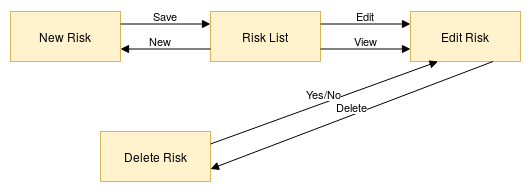
\includegraphics[width=1.0\textwidth]{Content/Domain/UC3RiskCRUDactivitydiagram.png}
	\caption{Activity Diagram \ac{UC}3 Risk CRUD}
	\label{fig:activityDiagramUC3}
\end{figure}

\paragraph*{Alternative Flows}\mbox{}\\

Reading a risk:  
\begin{itemize}
	\setlength\itemsep{-1.5em}
	\item The user is on the project overview site with all project risks
	\item By clicking on a risk a detail risk view is opened.
	\item For exiting the risk detail view a return button ("Close" button) is clicked.
\end{itemize}

Updating a risk: 
\begin{itemize}
	\setlength\itemsep{-1.5em}
	\item The user is on the project overview site with all project risks.
	\item By clicking on a risk a detail risk view is opened.
	\item On the detail view there is a pen button, enabling editing and changing the "Close" button to a "Save" button.
	\item When clicking the "Save" button the changes are syncronized with the server.
\end{itemize} 

Deleting a risk:
\begin{itemize}
	\setlength\itemsep{-1.5em}
	\item The user is on the project overview site with all project risks.
	\item By clicking on a risk a detail risk view is opened.
	\item By clicking a "Delete" button the risk is deleted. This behavior is changed in UC6 Risk Discussion \ref{sec:domainBbg}.
\end{itemize}

\paragraph*{Special Requirements and Preconditions}\mbox{}\\
The preconditions for this use case are:
\begin{enumerate}
	\setlength\itemsep{-1.5em}
	\item A project exists.
	\item The user is member of the project.
	\item The user has clicked the + button at the project overview page to add a new risk.
\end{enumerate}

\paragraph*{Postconditions and Persistance}\mbox{}\\
The postconditions for this use case are:
\begin{enumerate}
	\setlength\itemsep{-1.5em}
	\item The risk is immediately part of the projects risk table (this behavior is changed within UC6 Risk Discussion \ref{sec:domainBbg}).
\end{enumerate}

The persistence guidelines are: 

The risk form was completely or partly filled by the user. When the user tries to leave the page now, there should be a prompt for exiting. When the risk form is filled out and the button "Propose risk" is clicked a POST request syncs the status with the server.

\newpage
% UC4 ====================================================
\subsubsection{Use Case Specification: \ac{UC}4 Project risk overview}
\label{sec:domainBbe}

\paragraph*{Description}\mbox{}\\
Describe the functionality

\paragraph*{Screenshots}\mbox{}\\
Insert screenshots and shortly explain what can be seen
\begin{figure}[h] 
	\centering
	
\includegraphics[width=0.1\textwidth]{Content/Domain/placeholder.png}
	\caption{Use Case X: Detail}
	\label{fig:label4}
\end{figure}

\paragraph*{Basic Flow} \mbox{}\\

Describe the most common path through this use case

\subparagraph{Activity Diagram}\mbox{}\\
\begin{figure}[h]
	\centering
	
\includegraphics[width=0.1\textwidth]{Content/Domain/placeholder.png}
	\caption{Activity Diagram Use Case X}
	\label{fig:label44}
\end{figure}

\paragraph*{Alternative Flows}\mbox{}\\
What can go wrong :D

\paragraph*{Special Requirements and Preconditions}\mbox{}\\
Where does the user come from, what does he have to do before he gets here

\paragraph*{Postconditions and Persistance}\mbox{}\\
What has changed and how do we make sure the change persists?

\newpage
% UC5 ====================================================
\subsubsection{Use Case Specification: \ac{UC}5 Risk Pool}
\label{sec:domainBbf}

\paragraph*{Description}\mbox{}\\
Describe the functionality

\paragraph*{Screenshots}\mbox{}\\
Insert screenshots and shortly explain what can be seen
\begin{figure}[h] 
	\centering
	
\includegraphics[width=0.1\textwidth]{Content/Domain/placeholder.png}
	\caption{Use Case X: Detail}
	\label{fig:label5}
\end{figure}

\paragraph*{Basic Flow} \mbox{}\\

Describe the most common path through this use case

\subparagraph{Activity Diagram}\mbox{}\\
\begin{figure}[h]
	\centering
	
\includegraphics[width=0.1\textwidth]{Content/Domain/placeholder.png}
	\caption{Activity Diagram Use Case X}
	\label{fig:label55}
\end{figure}

\paragraph*{Alternative Flows}\mbox{}\\
What can go wrong :D

\paragraph*{Special Requirements and Preconditions}\mbox{}\\
Where does the user come from, what does he have to do before he gets here

\paragraph*{Postconditions and Persistance}\mbox{}\\
What has changed and how do we make sure the change persists?

\newpage
% UC6 ====================================================
\subsubsection{Use Case Specification: \ac{UC}6 Risk Discussion}
\label{sec:domainBbg}

\paragraph*{Description}\mbox{}\\
Describe the functionality

\paragraph*{Screenshots}\mbox{}\\
Insert screenshots and shortly explain what can be seen
\begin{figure}[h] 
	\centering
	
\includegraphics[width=0.1\textwidth]{Content/Domain/placeholder.png}
	\caption{Use Case X: Detail}
	\label{fig:label6}
\end{figure}

\paragraph*{Basic Flow} \mbox{}\\

Describe the most common path through this use case

\subparagraph{Activity Diagram}\mbox{}\\
\begin{figure}[h]
	\centering
	
\includegraphics[width=0.1\textwidth]{Content/Domain/placeholder.png}
	\caption{Activity Diagram Use Case X}
	\label{fig:label66}
\end{figure}

\paragraph*{Alternative Flows}\mbox{}\\
What can go wrong :D

\paragraph*{Special Requirements and Preconditions}\mbox{}\\
Where does the user come from, what does he have to do before he gets here

\paragraph*{Postconditions and Persistance}\mbox{}\\
What has changed and how do we make sure the change persists?

\newpage
% UC7 ====================================================
\subsubsection{Use Case Specification: \ac{UC}7 Risk Monitoring}
\label{sec:domainBbh}

\paragraph*{Description}\mbox{}\\
Describe the functionality

\paragraph*{Screenshots}\mbox{}\\
Insert screenshots and shortly explain what can be seen
\begin{figure}[h] 
	\centering
	
\includegraphics[width=0.1\textwidth]{Content/Domain/placeholder.png}
	\caption{Use Case X: Detail}
	\label{fig:label7}
\end{figure}

\paragraph*{Basic Flow} \mbox{}\\

Describe the most common path through this use case

\subparagraph{Activity Diagram}\mbox{}\\
\begin{figure}[h]
	\centering
	
\includegraphics[width=0.1\textwidth]{Content/Domain/placeholder.png}
	\caption{Activity Diagram Use Case X}
	\label{fig:label77}
\end{figure}

\paragraph*{Alternative Flows}\mbox{}\\
What can go wrong :D

\paragraph*{Special Requirements and Preconditions}\mbox{}\\
Where does the user come from, what does he have to do before he gets here

\paragraph*{Postconditions and Persistance}\mbox{}\\
What has changed and how do we make sure the change persists?

\newpage
% UC8 ====================================================
\subsubsection{Use Case Specification: \ac{UC}8 Risk Response Management}
\label{sec:domainBbi}

\paragraph*{Description}\mbox{}\\
Describe the functionality

\paragraph*{Screenshots}\mbox{}\\
Insert screenshots and shortly explain what can be seen
\begin{figure}[h] 
	\centering
	
\includegraphics[width=0.1\textwidth]{Content/Domain/placeholder.png}
	\caption{Use Case X: Detail}
	\label{fig:label8}
\end{figure}

\paragraph*{Basic Flow} \mbox{}\\

Describe the most common path through this use case

\subparagraph{Activity Diagram}\mbox{}\\
\begin{figure}[h]
	\centering
	
\includegraphics[width=0.1\textwidth]{Content/Domain/placeholder.png}
	\caption{Activity Diagram Use Case X}
	\label{fig:label88}
\end{figure}

\paragraph*{Alternative Flows}\mbox{}\\
What can go wrong :D

\paragraph*{Special Requirements and Preconditions}\mbox{}\\
Where does the user come from, what does he have to do before he gets here

\paragraph*{Postconditions and Persistance}\mbox{}\\
What has changed and how do we make sure the change persists?



TODO: INSERT USE CASES CONTEXT

\subsection{Requirements}
\label{sec:domainBc}
Couldn't find a better translation for "Anspruch" :/
Describes which 'Ansprüche' we have regarding the following categories:
\subsubsection{Usability}
\label{sec:domainBca}
\subsubsection{Reliability}
\label{sec:domainBcb}
\subsubsection{Performance}
\label{sec:domainBcc}
\subsubsection{Supportability}
\label{sec:domainBcd}

\subsection{Design Constraints}
\label{sec:domainBd}
Where does our software run? Where does it not? Which functions cannot be covered and why? Which conditions are required to use the software? Stuff like that

\subsection{Interfaces}
\label{sec:domainBe}
\subsubsection{User Interfaces}
\label{sec:domainBea}
Describe the views the software will have
\subsubsection{Further Interfaces}
\label{sec:domainBeb}
Software, Hardware and Communcation Interfaces... expand subsubsections if necessary
